\begin{center}
	
\end{center}\chapter{Phyisical Background }
\label{Phyisical Background}
\textit{This chapter discusses the theoretical framework related to graphene and GNRs and the importance of two-dimensional materials. It is currently a very well-studied topic, so interesting properties that have real applications in the field of electronics will be discussed, as well as the remarkable advances in the synthesis of graphene and GNRs.
}
\vfill
\minitoc\newpage

\section{Introduction to graphene}
\vspace{-1cm}
Graphene is defined as a novel two-dimensional sheet of atomic thickness which is organized in a hexagonal honeycomb lattice of $sp2$-hybridized carbon atoms (a 2s orbital is mixed with two of the 2p orbitals and a total of 3 hybrid orbitals can form covalent bonds, called $\sigma$ bonds with neighboring carbon atoms).  It has been extensively invesgated since Geim and Novoselov first isolated it by performing mechanical exfoliation based on repeated peeling of highly oriented pyrolyzed graphite. For their pioneering work, which revealed the exceptional physical properties of graphene, Geim and Novoselov were awarded the 2010 Nobel Prize in Physics. 
Graphene has extraordinary thermal, electronic and mechanical properties, which have generated great expectations for various applications like  energy storage , solar cells \cite{singh2015graphene} and conversion, biosensors \cite{yang2015graphene,shao2010graphene}, biocompatible materials \cite{pinto2013graphene}, batteries \cite{kucinskis2013graphene}, optoelectronics, electronics \cite{schwierz2010graphene,chee2016flexible,li2012review} and the latter is still facing challenges\cite{mullen2017polyphenylenes}.  To date it has been extensively researched and a large number of papers have been published showing evidence of its properties and thus applications. 
\begin{figure}
	\centering
	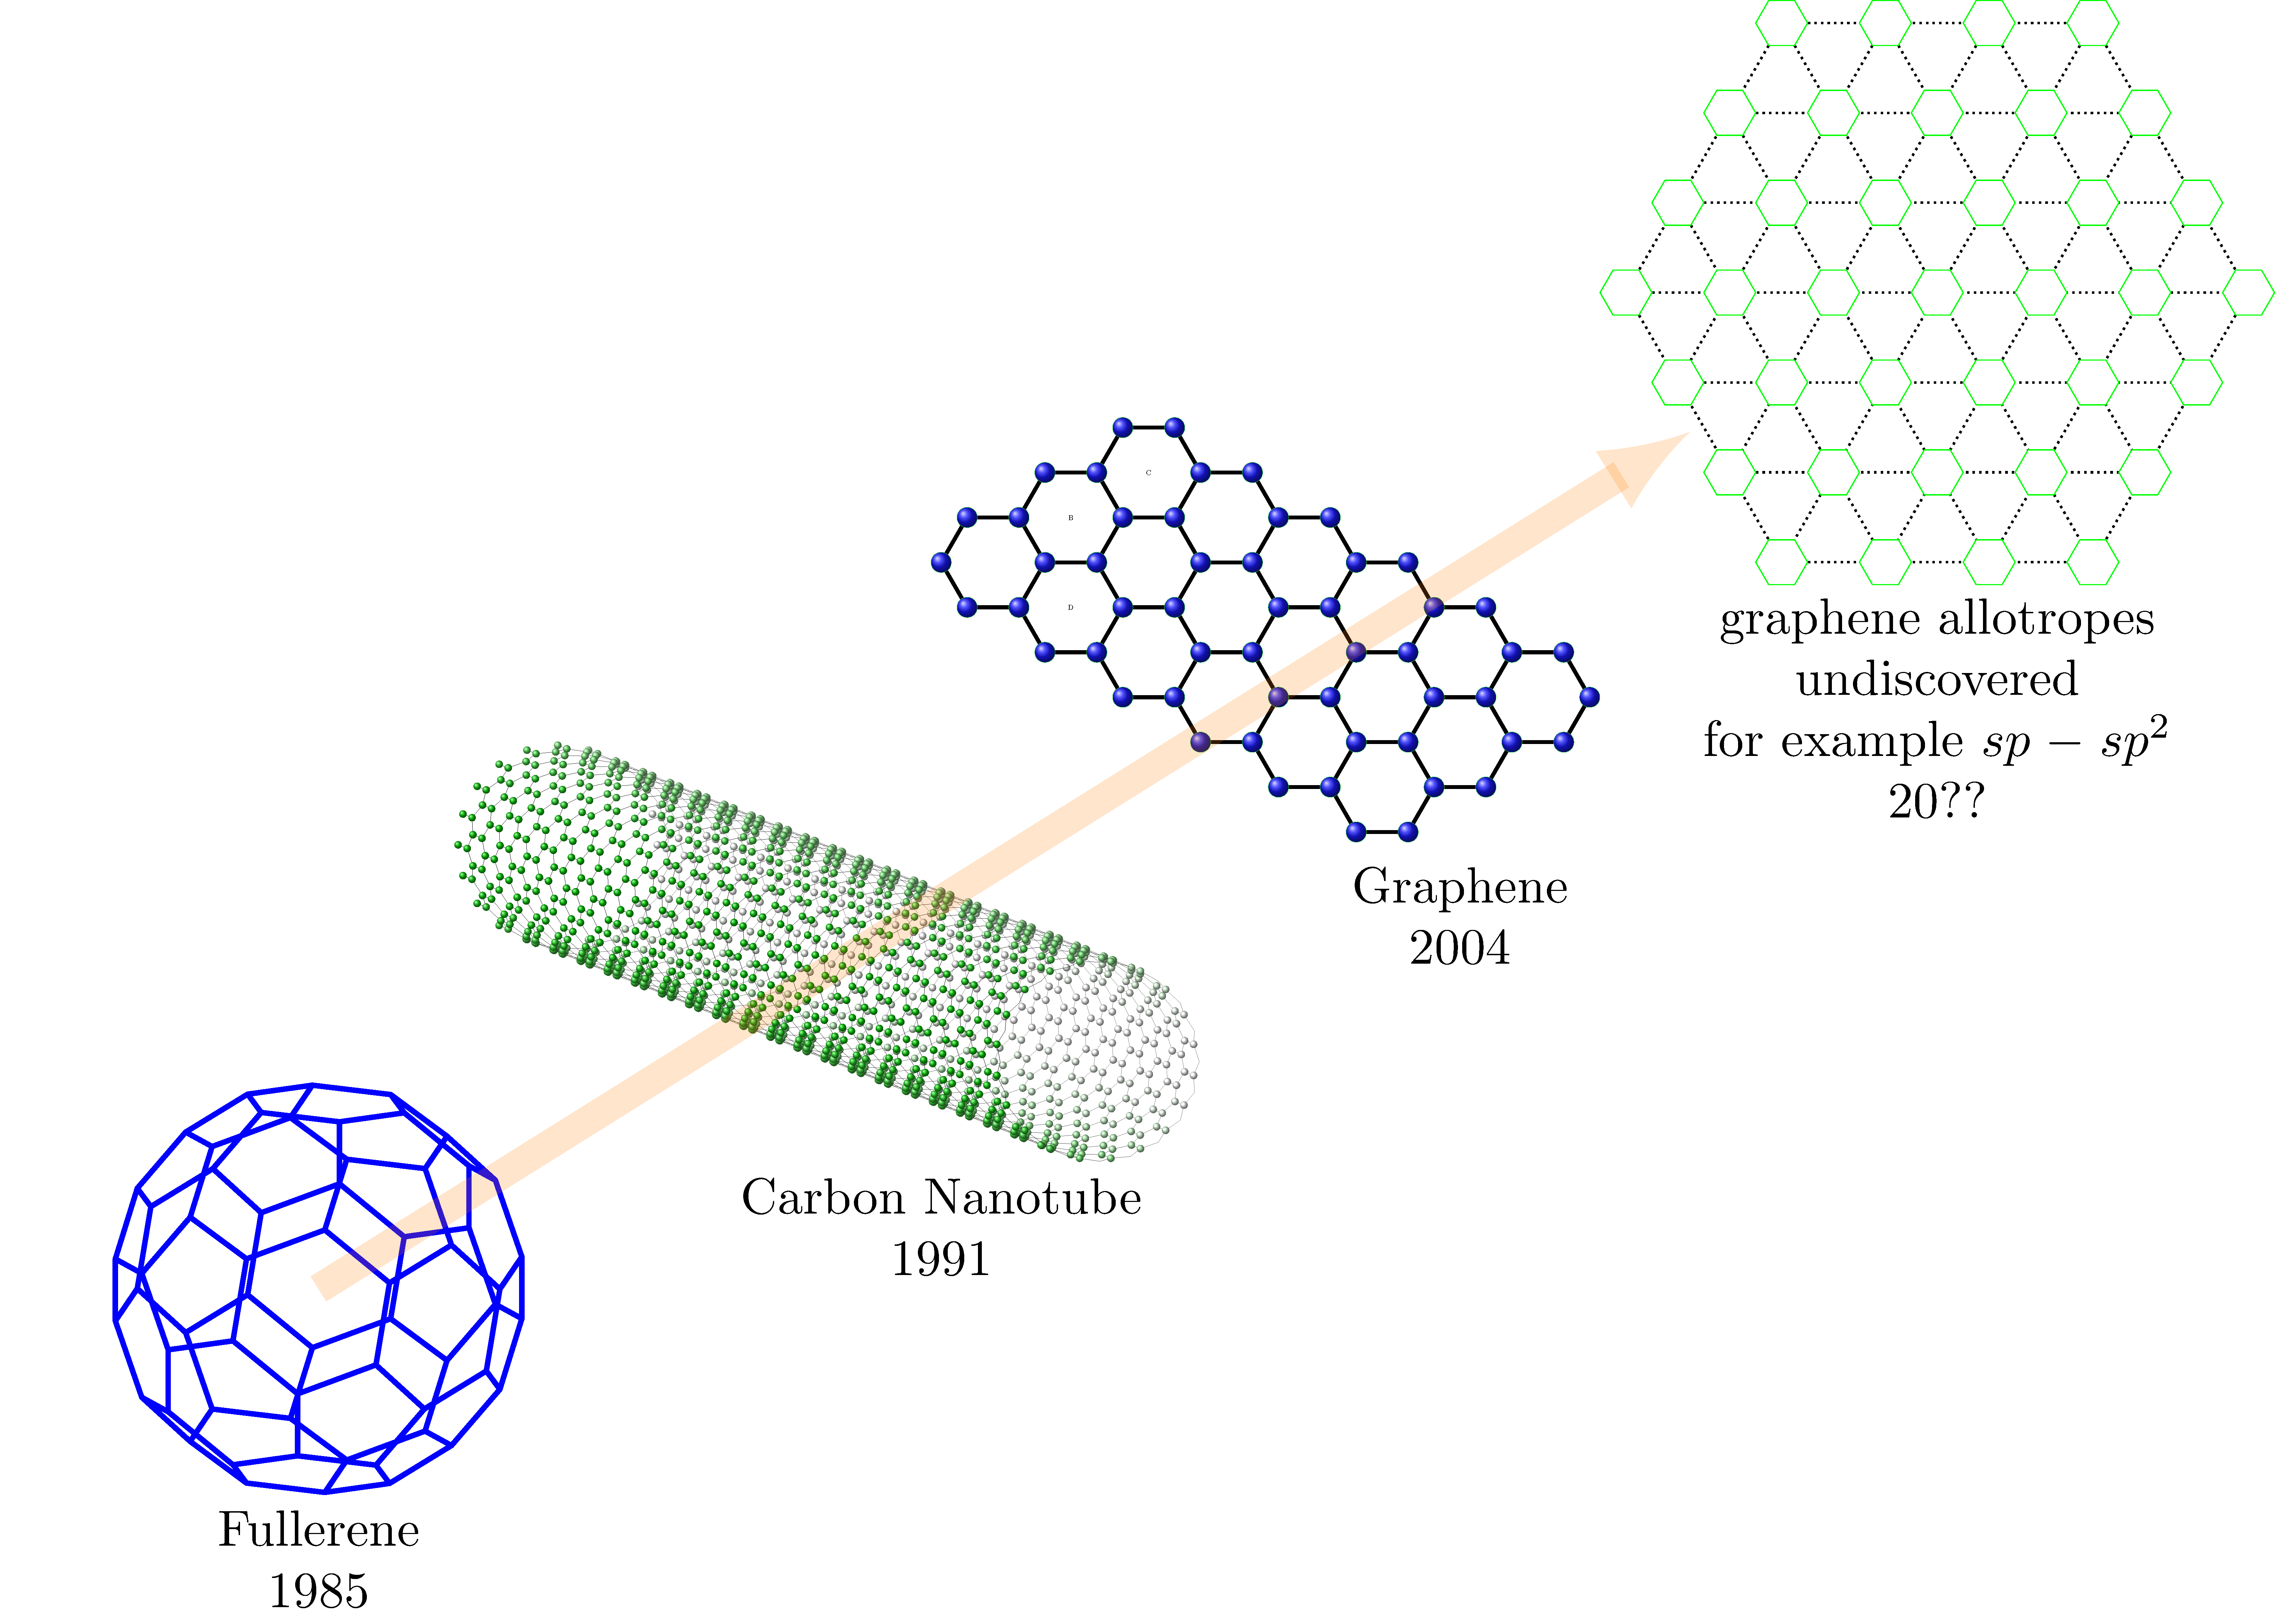
\includegraphics[width=0.8\linewidth]{FIGURES/Introduction/Intro_Fig3/Intro_Fig3}
	\caption{Carbon allotrope timeline}
	\label{fig:introfig32}
\end{figure}
\\
Given the electronic structure of graphene there are some applications that are not possible, a clear example is when you require a device you need to have an off-on process and that is why semiconductors (considerable gap) are optimal for these technological applications, however graphene has no gap and this makes it impossible to stop the flow of current so it is practically impossible to turn off at any reasonable temperature because in graphene large populations of carriers are easily produced by thermal energy and fluctuations. It is then that arises the search to induce a band gap with these graphene structures has been done much research in this area and we can mention some ways to open the gap in these structures i) applying uniaxial strain \cite{ni2008uniaxial}  ii) by dopants however this modifies the properties of graphene itself as it is a modification in the mobility of the same, iii)Graphene can grow epitaxially on SiC to form ribbons (GNRs) with widths controlled by growth conditions and post-growth annealing procedures \cite{celis2016graphene,baringhaus2014exceptional,sprinkle2010scalable}. The band gap of GNRs is a function of the ribbon width and that is why controlled growth followed by reliable determination of properties such as width and thickness is of fundamental importance to tailor the properties of these nanostructures to specific applications\cite{flores2021optical}.

LA estructura se puede ver como una red trangular con una base de dos atomos por celda unitaria. Los vectores se describen de la siguiente manera: 

\begin{equation}
	a_{1}=\frac{a}{2}(3, \sqrt{3}), 
	a_{2}=\frac{a}{2}(3, -\sqrt{3}),
\end{equation}
 Donde $a\approx 1.42\AA$ y sus vectores de la red reciproca estan dados por 
 \begin{equation}
	b_{1}=\frac{2 \pi}{3a}(1, \sqrt{3}), b_{2}=\frac{2 \pi}{3a}(1,-\sqrt{3})
 \end{equation}

\begin{figure}[h!]
	\centering
	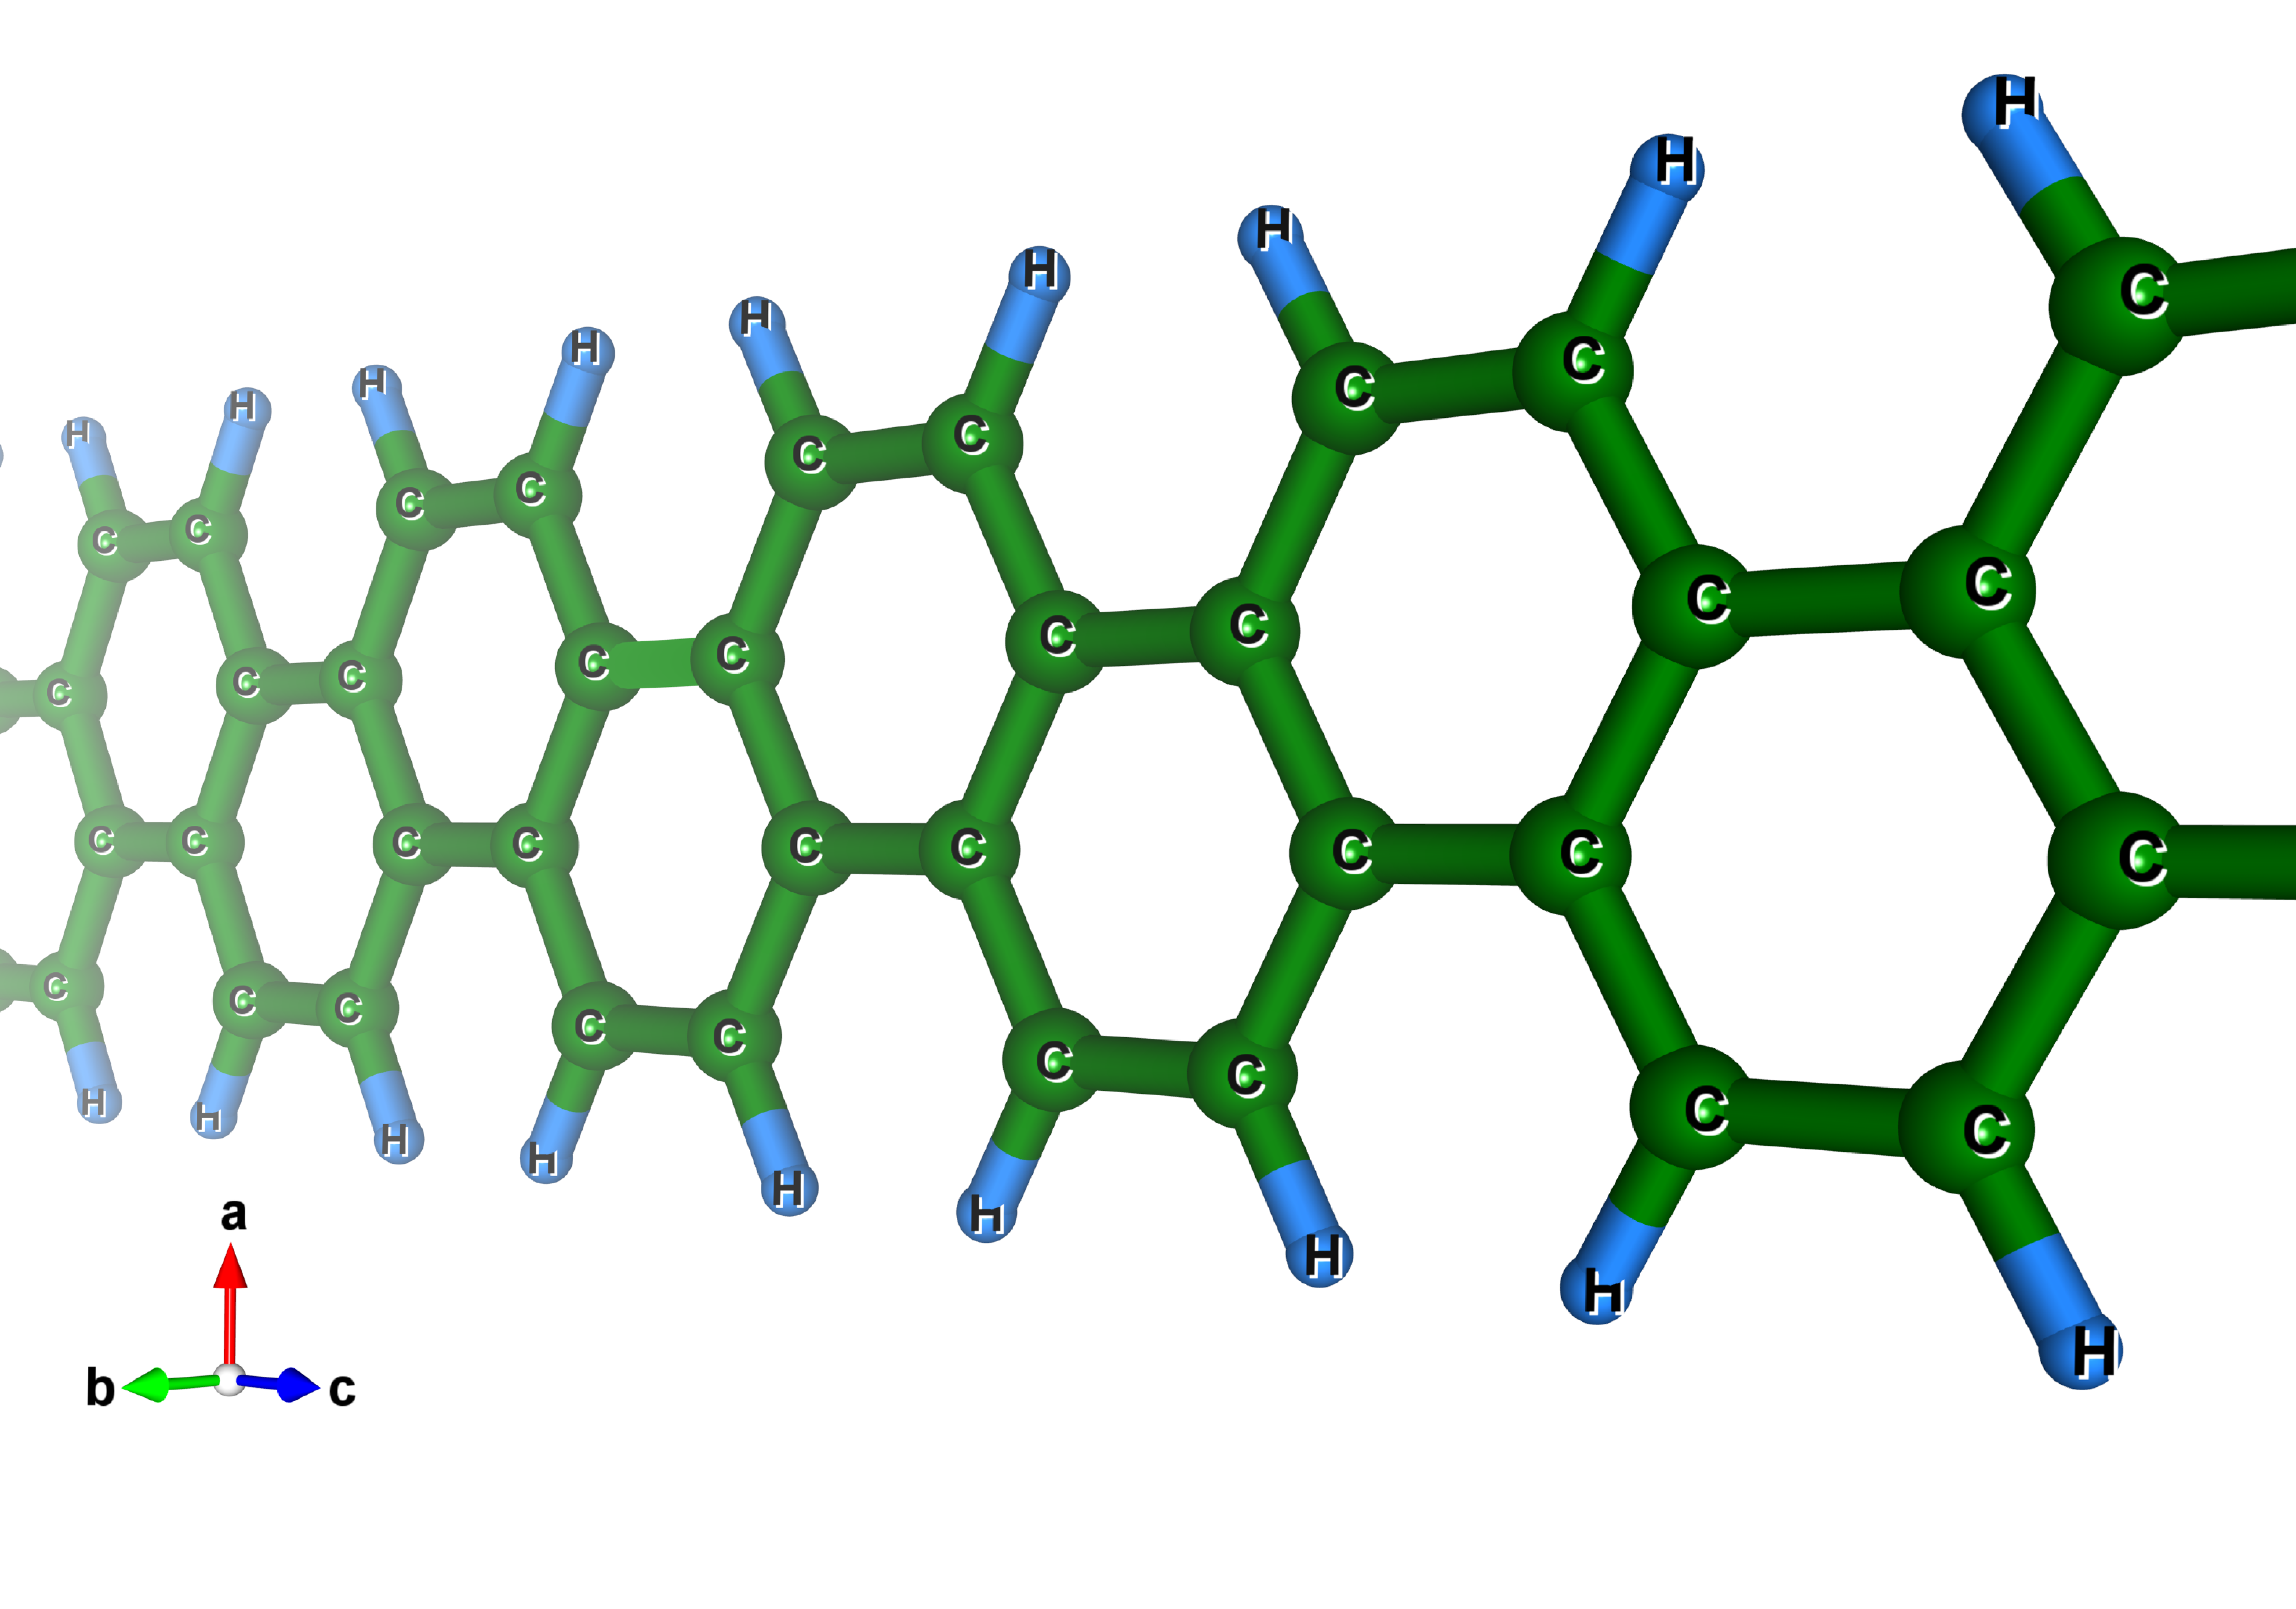
\includegraphics[width=0.80\linewidth]{FIGURES/Physical_Background/GNR-1}
	\caption{Structure of armchair GNRs, which are the ones we study throughout this thesis, are schematized with H at the end bonds. }
	\label{fig:introfig32}
\end{figure}


\subsection{Graphene Monolayers and Bilayers}
\vspace{-1cm}
The atomic structure of carbon allows it to be used in different configurations such as i) folded into fullerenes (0D), ii) rolled into nanotubes (1D), iii) stacked into graphite (3D). The carbon atoms of graphene are separated by an interatomic distance of $a=1.42\angstrom$ and the primitive cell of graphene is composed of two non-equivalent atoms. As for its electronic configuration it is very important to mention that the planar orbitals form the energetically stable and localized $\sigma$ bonds with the three nearest carbon atoms in the honeycomb lattice, and are responsible for most of the binding energy and elastic properties of the graphene layer so that the remaining 2pz orbitals have $\pi$ symmetry and the overlap of these orbital states between neighboring atoms plays an important role in the electronic properties of graphene.

\begin{figure}[H]
	\centering
	\includegraphics[width=0.5\textwidth]{example-image}
	\caption{a) Band structure of graphene with the respective projections in the $k_y$ and $k_x$ plane, the insight shows the linear dispersion is observed, i.e. near the point $K$ and $K\prime$ (Dirac Point), b)Honeycomb lattice of graphene, showing the unit cell corresponding to two non-equivalent atoms A and B.
	}
	\label[figure]{}
\end{figure}



\subsubsection{Phonons in graphene}
\subsection{Graphene Nanoribbons}
\vspace{-1cm}
In the case of GNRs it is worth mentioning that many of their essential properties have been conducted by the tight-binding model\cite{nakada1996edge,sohmen1992electronic}and the first-principles method\cite{son2006half}. In the former model GNRs in armchair configuration are predicted to be metals and in the latter they are semiconductors for $N_A=3I+2$ where $N_A$ is the number of dimer lines along the transverse direction corresponding to the electronic states of monolayer graphene in the presence of open boundary conditions. The energy gaps are predicted to be inversely proportional to the width of the nano-ribbons, clearly indicating the quantum confinement effect. In addition, the electronic properties are sensitive to the change in the structure of the edges recalling that there are two configurations i)armchair which are the already described in this work and ii) and zigzag\cite{lin2018structure}
\subsubsection{Nanoribbon structure}

\subsubsection{Phonons in nanoribbons}

\section{Most relevant properties}




















\subsection{Electronic properties}

\section{Theoretical and numerical DFT}
\vspace{-1cm}
The objective in this section of the thesis is to use these existing computational tools to correlate with the experimental results.



\begin{figure}[h!]
	\centering
	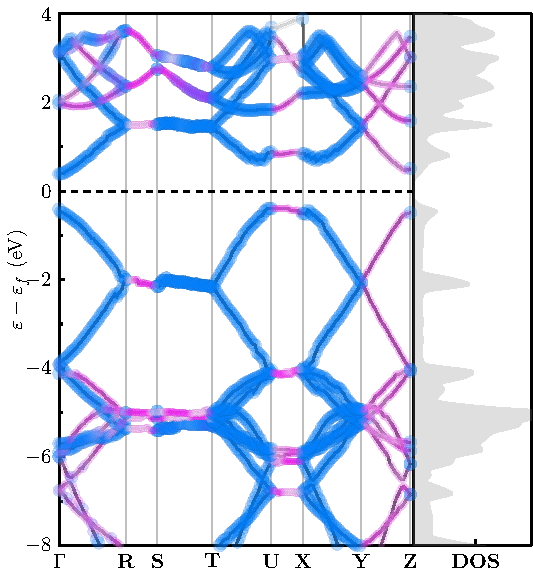
\includegraphics[width=0.80\linewidth]{FIGURES/Physical_Background/PLOT-GNRS007}
	\caption{Structure of armchair GNRs, which are the ones we study throughout this thesis, are schematized with H at the end bonds. }
	\label{fig:introfig32}
\end{figure}


\begin{figure}[h!]
	\centering
	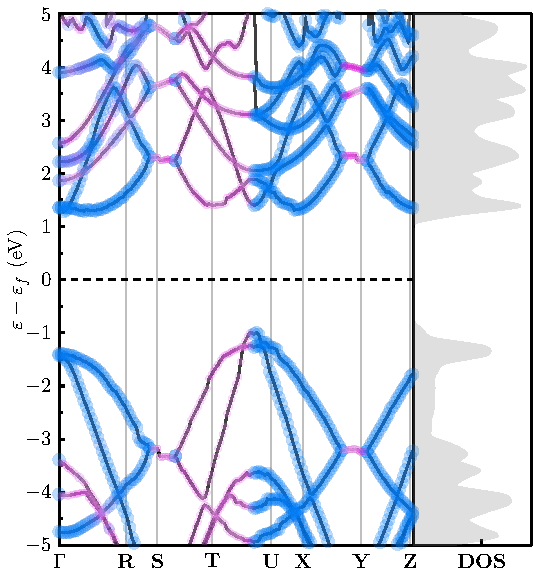
\includegraphics[width=0.80\linewidth]{FIGURES/Physical_Background/PLOT-GNRS008}
	\caption{Structure of armchair GNRs, which are the ones we study throughout this thesis, are schematized with H at the end bonds. }
	\label{fig:introfig32}
\end{figure}





\section{Importance of the optical characterization}
\vspace{-1cm}
In addition to the interest of graphene layers (from 1 layer up to 10), graphene nanostructures such as the ones we have studied which are GNRs show a wide interest for various potential electronic applications. It has been studied that nanostructures can offer a direct band gap due to quantum confinement of charge carriers and that it depends on both lateral width and termination which is required for switching devices and even for DNA sequencing tools. 



\section{Applications}

